\documentclass[thesis.tex]{subfiles}
\begin{document}

\chapter{Related Work}
\todo[inline]{todo: add rendering stuff?}
\section{Fourier Transform} \label{fourier_transform}

In mathematics the fourier transform \cite{nixon2012feature} is a function that approximates a one-dimensional signal in the time domain by a sum of sine and cosine functions with different frequencies. The result is then in the frequency domain. This means the signal is represented by frequencies, amplitudes and phases.
\\ 
It is possible to visualize how the fourier transform works: Consider going along the outline of a circle over time. While going along on the outline of the circle we construct a two-dimensional function in the following way. We use the elapsed time as the x-values of the constructed function. For the y-values of the function we use the y-values of the position on the circle outline at each timepoint. The resulting function is a sine wave as seen in \ref{fig:fourier}. There are three parameters that can be adjusted in this process: the radius of the circle, the speed at which we go along the outline of the circle, and the starting position on the outline of the circle. \\
Sine waves can be defined by a frequency, amplitude and phase. We will now show that we can arbitrarily change the frequency, amplitude and phase of the constructed sine wave by changing the three parameters of the circle. By changing the radius of the circle we change the amplitude of the constructed sine wave. Figure \ref{fig:fourier_radius} shows that the radius directly corresponds to the amplitude of the constructed sine wave. If we change the speed at which we go along the outline of the circle, we change the frequency of the resulting sine wave. In figure \ref{fig:fourier_speed} we doubled the speed at which we go along the outline of the circle compared to \ref{fig:fourier}. This results in a sine wave with double the frequency. Also, by changing the starting position on the outline of the circle, we can change the phase of the sine wave. \\
So far we only constructed simple sine waves. We can also construct more complex functions by using multiple circles: Instead of going along the outline of a single circle, we place a new circle on the outline of the previous circle. Each new circle moves along the outline of the previous circle. By repeating this, we can use an arbitrary number of circles. For the y-values of the constructed function, we then only use the y-values of the positions on the outline of the last circle. In figure \ref{fig:fourier_square} a square wave is approximated by using 4 circles. 
\\
The fourier transform works by finding the values of the three parameters for each circle to optimally approximate a given one-dimensional function. In literature the circles are refered to as \textit{harmonic circles}. The fourier transform returns only two coefficients per harmonic circle, but the two coefficients can be used to compute all three parameters. In this thesis we call the set of fourier coefficients that describe a single harmonic circle a \textit{harmonic}. 
 \\ One important property of the fourier transform is that signals can be approximated arbitrarily well by specfying the number of harmonics that are used \cite{nixon2012feature}. The more harmonics are used for the approximation, the better the approximation \cite{nixon2012feature}. Many common signals can be perfectly reconstructed using the fourier transform, but some, for example the square wave that we approximated in figure \ref{fig:fourier_square}, need an infinite number of harmonics for perfect reconstruction.\\ 

\begin{figure}
\centering
	\begin{subfigure}[t]{\textwidth}
		\centering
		\includegraphics[width=\textwidth,clip, trim=0cm 2.5cm 0cm 3cm]{6sin(x)/Animation_0246.jpg}
		\caption{By going along the outline of a harmonic circle it is possible to construct a sine wave.}\label{fig:fourier}		
	\end{subfigure}
	\begin{subfigure}[t]{\textwidth}
		\centering
		\includegraphics[width=\textwidth,clip, trim=0cm 2.5cm 0cm 1cm]{3sin(x)/Animation_0246.jpg}
		\caption{Changing the radius of the harmonic circle changes the amplitude of the resulting sine wave. Compared to \ref{fig:fourier} the radius of the circle was halved and is now at three.}\label{fig:fourier_radius}		
	\end{subfigure}
	\begin{subfigure}[t]{\textwidth}
		\centering
		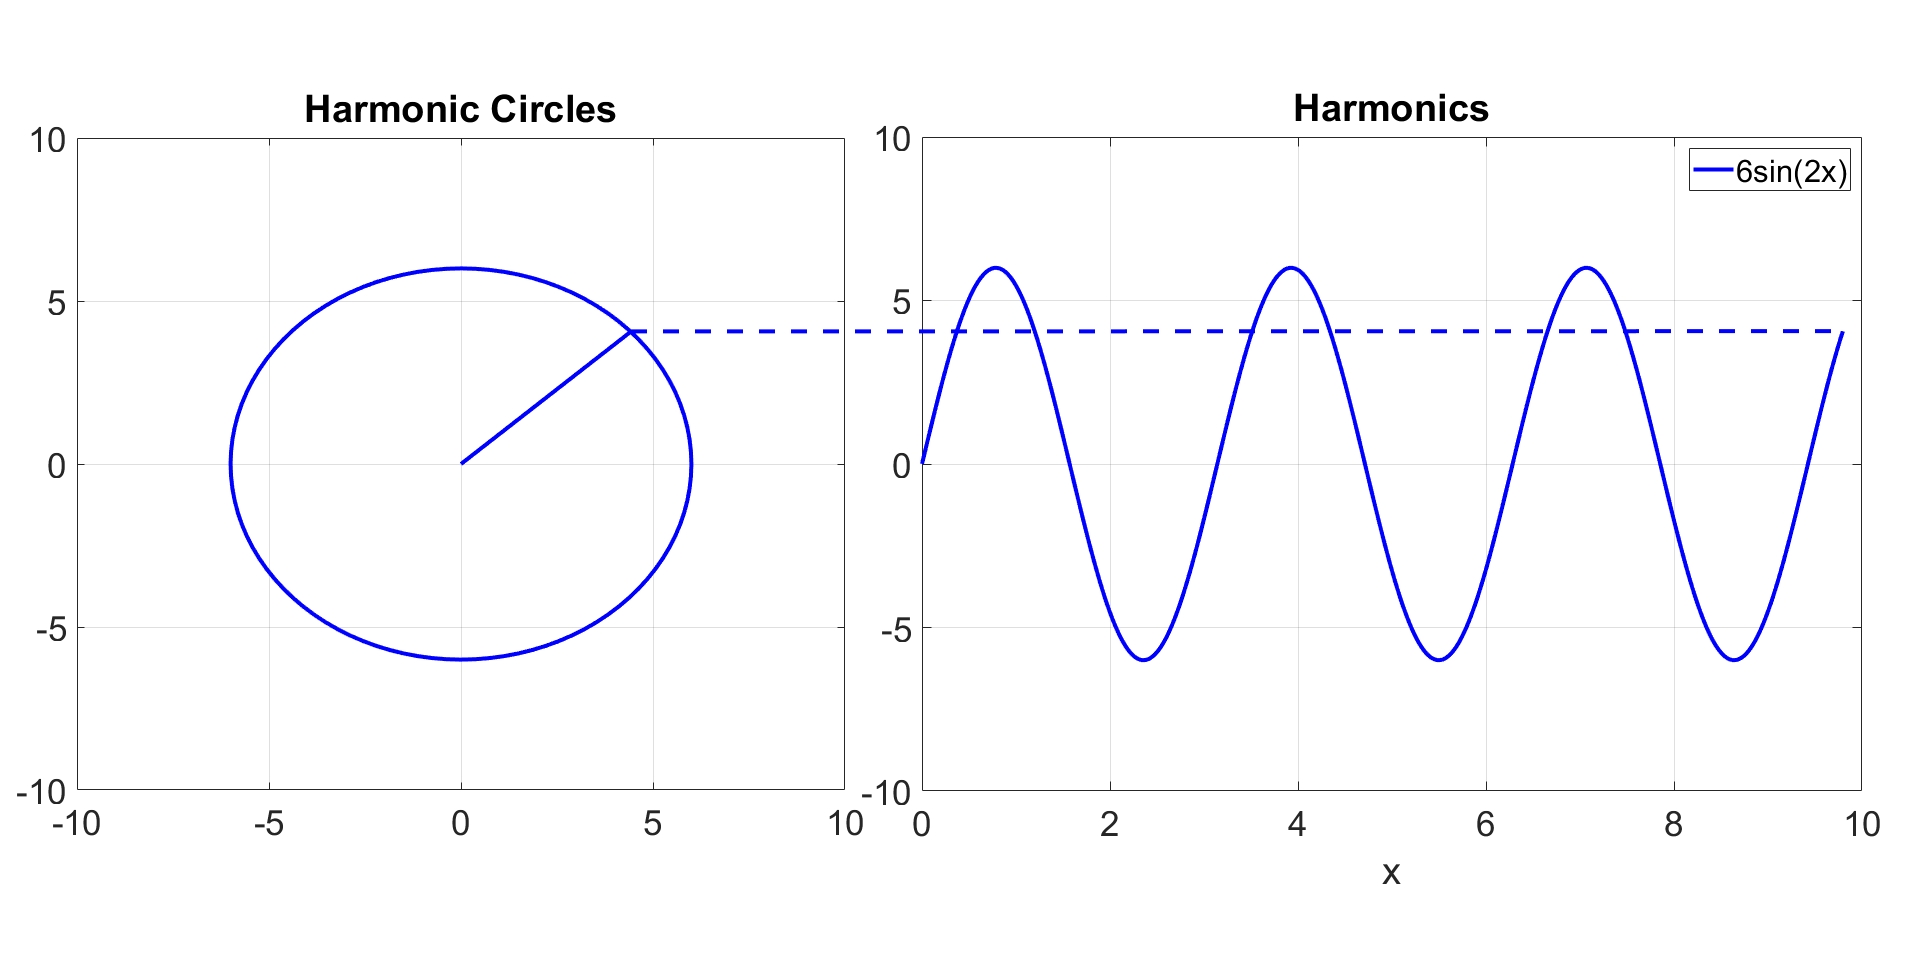
\includegraphics[width=\textwidth,clip, trim=0cm 2.5cm 0cm 1cm]{6sin(2x)/Animation_0344.jpg}
		\caption{Changing the speed at which we go along the outline of the harmonic circle changes the frequency of the resulting sine wave. Compared to \ref{fig:fourier} the speed at which we go along the outline of the circle was doubled which results in a doubled frequency.}\label{fig:fourier_speed}		
	\end{subfigure}
	\caption{}
\end{figure}
 \smallskip

%\begin{figure}[h]
%\centering
%\includegraphics[width=\textwidth]{6sin(x)/Animation_0246.jpg}
%\caption{By going along the outline of a circle it is possible to construct a sine wave.}
%\label{fig:fourier}
%\end{figure}
%
%\begin{figure}[h]
%\centering
%\includegraphics[width=\textwidth]{3sin(x)/Animation_0246.jpg}
%\caption{Changing the radius of the circle changes the amplitude of the resulting sine wave. Compared to \ref{fig:fourier} the radius of the circle was halved and is now at three.}
%\label{fig:fourier_radius}
%\end{figure}
%
%\begin{figure}[h]
%\centering
%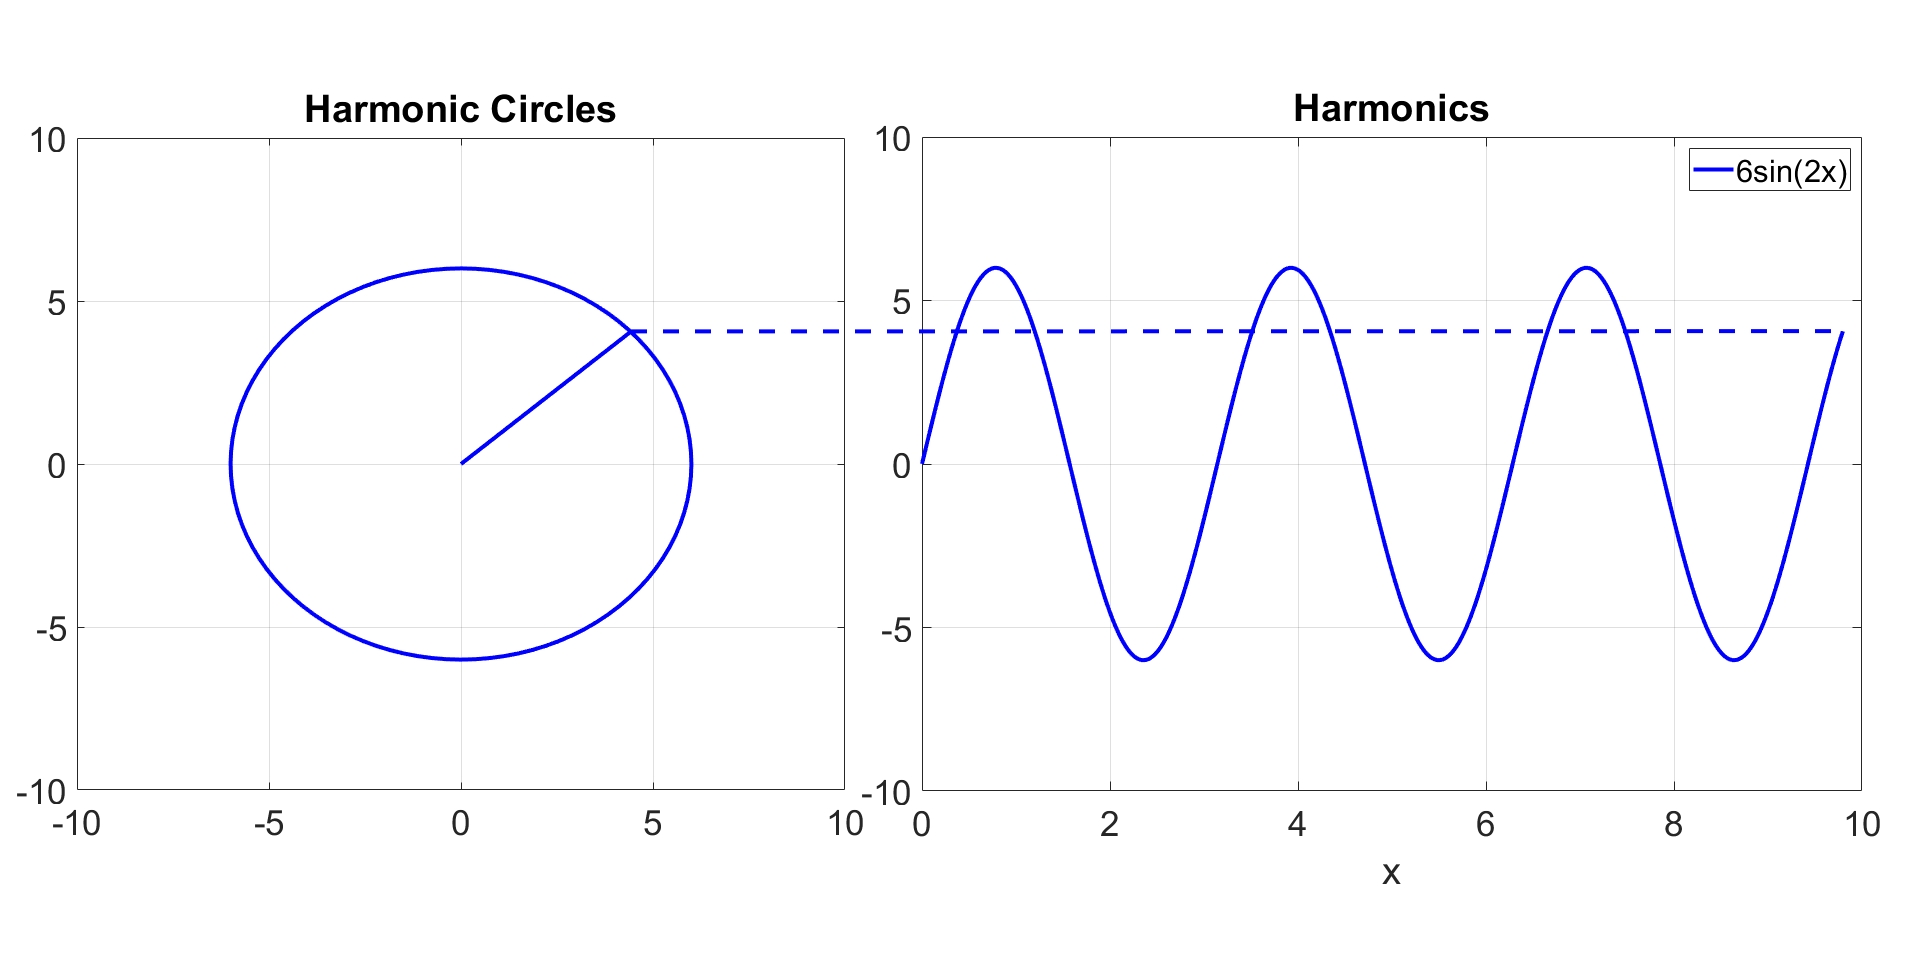
\includegraphics[width=\textwidth]{6sin(2x)/Animation_0344.jpg}
%\caption{Changing the speed at which we go along the outline of the circle changes the frequency of the resulting sine wave. Compared to \ref{fig:fourier} the speed at which we go along the outline of the circle was doubled which results in a doubled frequency.}
%\label{fig:fourier_speed}
%\end{figure}

\begin{figure}[h]
\centering
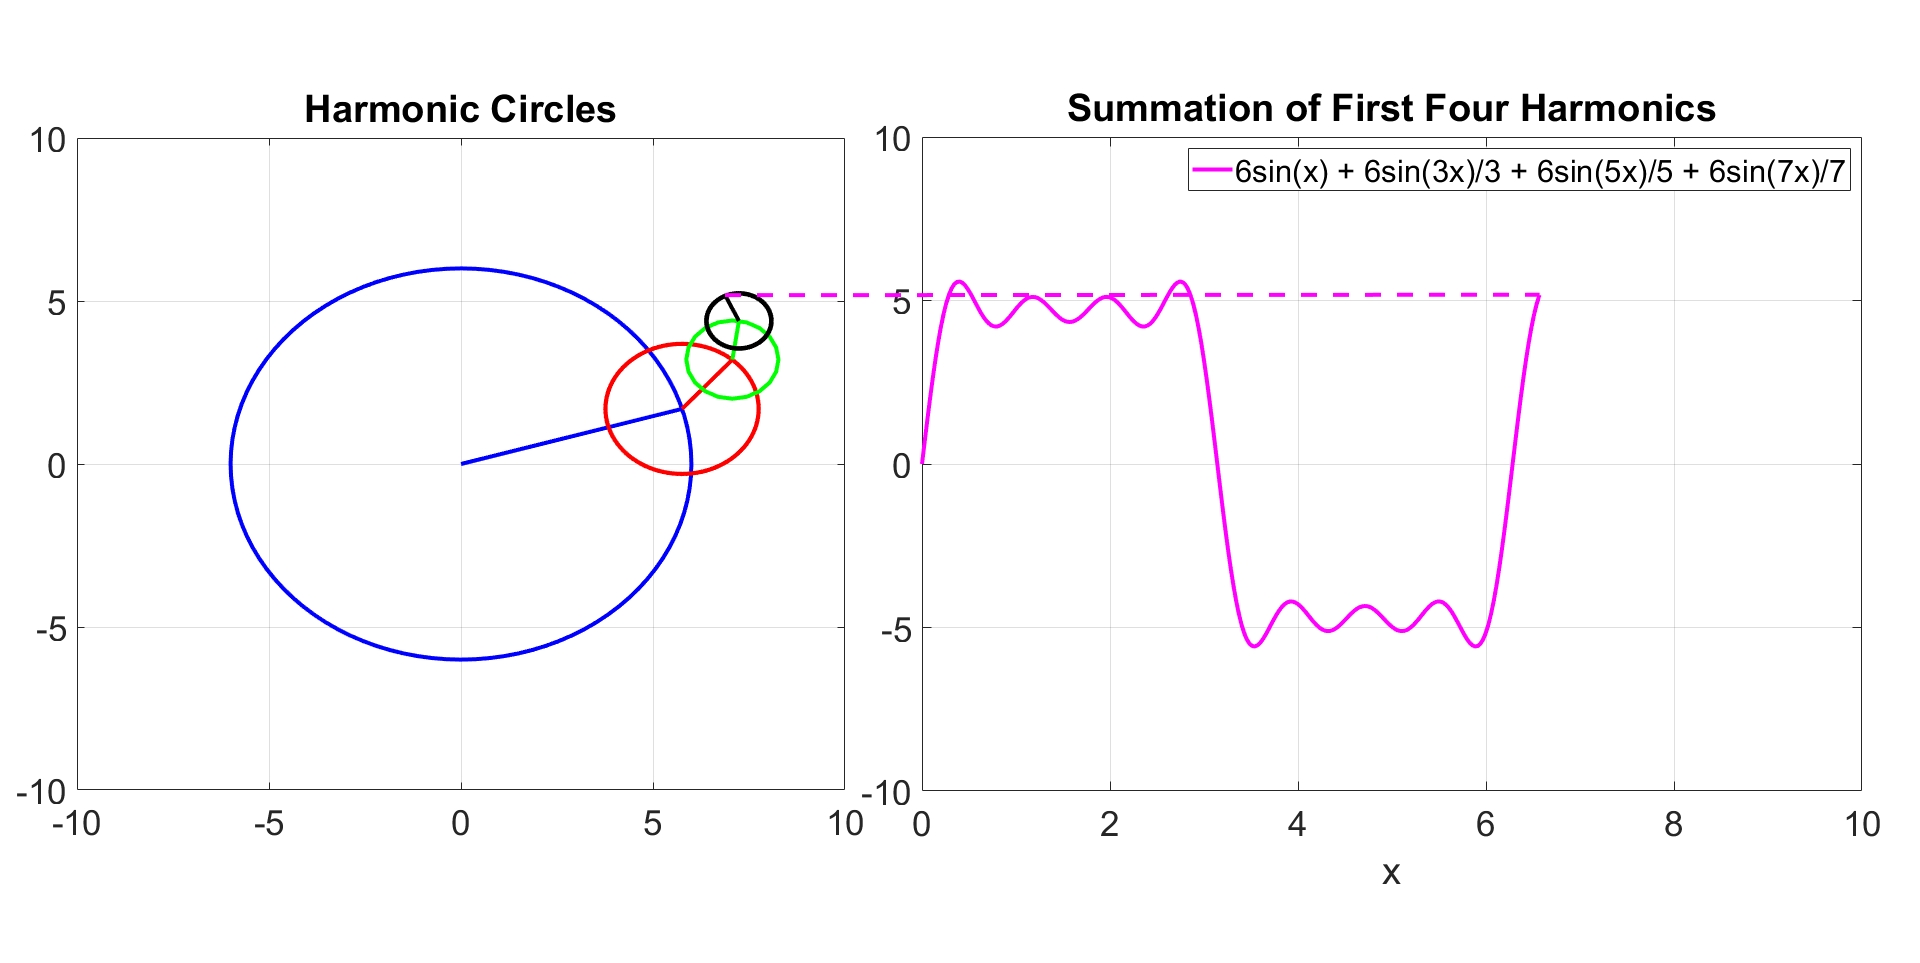
\includegraphics[width=\textwidth]{square_wave/Animation_0891.jpg}
\caption{More complex functions can be approximated by repeating the process recursively by using circles that go along the outline of the previous circle. In this figure 4 harmonic circles are used to appropximate a square wave.}
\label{fig:fourier_square}
\end{figure}

\subsection{Discrete Fourier Transform}
Several different versions of the fourier transform exist to handle different kinds of input signals. In practice signals usually are finite and discrete, because memory in computers is limited and cannot store an infinite amount of values. For such input signals the \textit{Discrete Fourier Transform} (DFT) can be used. The DFT is a version of the fourier transform that can handle discrete and finite signals. The DFT assumes a periodic input signal \cite{dspguide}. Also, the first coefficient computed by the DFT is called \textit{DC Component}. The DC component does not describe the shape of the signal. In this thesis we apply the fourier transform on closed contours, which are represented by periodic, discrete, and finite functions. This means the DFT is suited for this kind of input signals.
\newpage

\section{Contour-Tracing Algorithm} 
\label{contourtracingalgorithm}
A contour-tracing algorithmn can be used to extract the boundary of objects in an image. The boundary of an object is called it's contour. An overview of different approaches to contour tracing algorithmns is given in \cite{seo2016fast}. The authors also propose a new contour-tracing algorithmn that we use in this thesis. Therefore, in this section we focus on describing this particular contour-tracing algorithm.

The proposed algorithm is a pixel-following method. This means that it starts at a given pixel and tries to find the next contour pixel by checking the pixels in the local neighborhood. The order in which the neighborhood pixels are checked is defined by simple rules. \\ The algorithm keeps track of the current pixel position it is on and of an absolute direction. In the context of contour-tracing algorithms, this set of the current pixel position and a direction is called a \textit{Tracer}. 

\textbf{Direction of the Tracer}

The absolute direction of the tracer of this algorithm can be \textit{north}, \textit{east}, \textit{south}, or \textit{west}. The pixels that are checked are defined relative to this absolute direction. For example, if the direction is \textit{east}, then the pixel to the \textit{left} of the current pixel is the pixel above the current pixel. Depending on the position of the next contour pixel relative to the absolute direction, the absolute direction is updated throughout the algorithm by rotating it by 90 degrees counter-clockwise, or clockwise, or by flipping the direction. Figure \ref{fig:contour_tracing} shows how the direction is changed in all specific cases the algorithm can differentiate.

\newpage
\textbf{Tracing}

For initilization of the algorithm, the user has to provide the initial values for the tracer. This means the user has to provide a starting pixel position and an initial absolute direction. For the algorithm to work correctly the following two conditions have to be fullfilled:
\begin{enumerate}
\item{The starting pixel is a contour pixel.}
\item{The left-rear pixel relative to the starting pixel is not an inner-outer corner pixel.}
\label{starting_pixel_conditions}
\end{enumerate}
  
After initilization the algorithm works in two phases. These two phases are repeated until the current pixel is the starting pixel and the direction is the same as at the start of the algorithm. In the first phase the algorithm only checks the left and rear-left pixels. In the second phase, it only checks the front and front-left pixels. Figure \ref{fig:contour_tracing} shows all cases that can occur in both phases. The first row of the figure shows all cases that can occur in the first phase, while the second row shows all cases that can occur in the second phase of the algorithm. The figure also shows for each case in which order the pixels are traced and what the respective direction at each contour pixel is. \\
It should be noticed that only pixels in the front, rear or left of the current direction are ever checked. However, if none of the checked pixels is a contour pixel, the direction is flipped (see figure \ref{contourTracingH}), which means that the pixels that were not checked in this iteration, because they are on the right side of the current pixel, will be on the left side in the next iteration.  \\ \\
The main reason why we chose this particular contour-tracing algorithm is because it does not have the problems of other traditional contour-tracing algorithms. In the paper of this algorithm, the authors analyzed traditional contour-tracing algorithms and found problems for each of them such as missed contour pixels, premature termination, or repeated tracing of the same pixels due to problems with defining a stopping criterion. \\
Another reason for choosing this algorithm is it's ability to classify contour pixels. Figure \ref{fig:contour_tracing} shows the cases in which a pixel can be classified as an \textit{inner}, \textit{inner-outer}, \textit{straight line} or \textit{outer} contour pixel. We think we can take advantage of this ability to classify pixels for example to create the vertex chain code which also differentiates between straight contour elements, outer-corner, and  inner-corner vertices.


\newcommand{\figcontourwidth}{3.5}
\newcommand{\figcontourfirstOffset}{0}
\newcommand{\figcontousecondOffset}{4.5}
\newcommand{\figcontouthirdOffset}{9}
\newcommand{\figcontoufourthOffset}{13.5}
\newcommand{\figcontousecondRowYOffset}{4.5}	

\newcommand\ContourPhaseOneCaseOne{
\begin{tikzpicture}
%phase 1 case 1
	\filldraw [fill=gray!50, draw=black, very thick] (\figcontourfirstOffset,0) rectangle (\figcontourfirstOffset + \figcontourwidth/2, \figcontourwidth/2); %rear-left pixel
	\filldraw [fill=gray!50, draw=black, very thick] (\figcontourfirstOffset, \figcontourwidth/2) rectangle (\figcontourfirstOffset + \figcontourwidth/2, \figcontourwidth); % left pixel
	\filldraw [fill=gray!50, draw=black, very thick] (\figcontourfirstOffset + \figcontourwidth/2, \figcontourwidth/2) rectangle (\figcontourfirstOffset + \figcontourwidth, \figcontourwidth); % current pixel
	\draw [draw=black, very thick] (\figcontourfirstOffset + \figcontourwidth/2,0) rectangle (\figcontourfirstOffset + \figcontourwidth, \figcontourwidth/2); % rear pixel
	
%arrows
	\draw[draw=black, line width=3.0pt, {*[fill=darkgreen!60]}-Latex] (\figcontourfirstOffset + \figcontourwidth/2 + \figcontourwidth/4, \figcontourwidth/2 + \figcontourwidth/12) -- (\figcontourfirstOffset + \figcontourwidth - \figcontourwidth/4, \figcontourwidth - \figcontourwidth/16);
\draw[draw=black, line width=3.0pt, -Latex](\figcontourfirstOffset + \figcontourwidth/2 - \figcontourwidth/12,  \figcontourwidth/2 + \figcontourwidth/4) -- (\figcontourfirstOffset + \figcontourwidth/16, \figcontourwidth/2 + \figcontourwidth/4);
\draw[draw=black, line width=3.0pt, -Latex] (\figcontourfirstOffset + \figcontourwidth/2 - \figcontourwidth/4, \figcontourwidth/2 - \figcontourwidth/12) -- (\figcontourfirstOffset + \figcontourwidth/4,0 + \figcontourwidth/16);

%dashed
\draw[draw=black, line width=1.5pt, dashed] (\figcontourfirstOffset + \figcontourwidth - \figcontourwidth/4, \figcontourwidth - \figcontourwidth/16) -- (\figcontourfirstOffset + \figcontourwidth/2 - \figcontourwidth/12,  \figcontourwidth/2 + \figcontourwidth/4);
\draw[draw=black, line width=1.5pt, dashed] (\figcontourfirstOffset + \figcontourwidth/16, \figcontourwidth/2 + \figcontourwidth/4) -- (\figcontourfirstOffset + \figcontourwidth/2 - \figcontourwidth/4, \figcontourwidth/2 - \figcontourwidth/12);
\end{tikzpicture}
}
\newcommand\ContourPhaseOneCaseTwo{
\begin{tikzpicture}
%phase 1 case 2
	\filldraw [fill=gray!50, draw=black, very thick] (\figcontousecondOffset,0) rectangle (\figcontousecondOffset + \figcontourwidth/2, \figcontourwidth/2); %rear-left pixel
	\filldraw [fill=white, draw=black, very thick] (\figcontousecondOffset, \figcontourwidth/2) rectangle (\figcontousecondOffset + \figcontourwidth/2, \figcontourwidth); % left pixel
	\filldraw [fill=gray!50, draw=black, very thick] (\figcontousecondOffset + \figcontourwidth/2, \figcontourwidth/2) rectangle (\figcontousecondOffset + \figcontourwidth, \figcontourwidth); % current pixel
	\draw [draw=black, very thick] (\figcontousecondOffset + \figcontourwidth/2,0) rectangle (\figcontousecondOffset + \figcontourwidth, \figcontourwidth/2); % rear pixel

%arrows
	\draw[draw=black, line width=3.0pt, {*[fill=darkgreen!60]}-Latex] (\figcontousecondOffset + \figcontourwidth/2 + \figcontourwidth/4, \figcontourwidth/2 + \figcontourwidth/12) -- (\figcontousecondOffset + \figcontourwidth - \figcontourwidth/4, \figcontourwidth - \figcontourwidth/16);
\draw[draw=black, line width=3.0pt, -Latex] (\figcontousecondOffset + \figcontourwidth/2 - \figcontourwidth/4, \figcontourwidth/2 - \figcontourwidth/12) -- (\figcontousecondOffset + \figcontourwidth/4,0 + \figcontourwidth/16);

%dashed
\draw[draw=black, line width=1.5pt, dashed] (\figcontousecondOffset + \figcontourwidth - \figcontourwidth/4, \figcontourwidth - \figcontourwidth/16) -- (\figcontousecondOffset + \figcontourwidth/2 - \figcontourwidth/4, \figcontourwidth/2 - \figcontourwidth/12);

\end{tikzpicture}
}

\newcommand\ContourPhaseOneCaseThree{
\begin{tikzpicture}
%phase 1 case 3
	\filldraw [fill=white, draw=black, very thick] (\figcontouthirdOffset,0) rectangle (\figcontouthirdOffset + \figcontourwidth/2, \figcontourwidth/2); %rear-left pixel
	\filldraw [fill=gray!50, draw=black, very thick] (\figcontouthirdOffset, \figcontourwidth/2) rectangle (\figcontouthirdOffset + \figcontourwidth/2, \figcontourwidth); % left pixel
	\filldraw [fill=gray!50, draw=black, very thick] (\figcontouthirdOffset + \figcontourwidth/2, \figcontourwidth/2) rectangle (\figcontouthirdOffset + \figcontourwidth, \figcontourwidth); % current pixel
	\draw [draw=black, very thick] (\figcontouthirdOffset + \figcontourwidth/2,0) rectangle (\figcontouthirdOffset + \figcontourwidth, \figcontourwidth/2); % rear pixel

%arrows
	\draw[draw=black, line width=3.0pt, {*[fill=darkgreen!60]}-Latex] (\figcontouthirdOffset + \figcontourwidth/2 + \figcontourwidth/4, \figcontourwidth/2 + \figcontourwidth/12) -- (\figcontouthirdOffset + \figcontourwidth - \figcontourwidth/4, \figcontourwidth - \figcontourwidth/16);
\draw[draw=black, line width=3.0pt, -Latex](\figcontouthirdOffset + \figcontourwidth/2 - \figcontourwidth/12,  \figcontourwidth/2 + \figcontourwidth/4) -- (\figcontouthirdOffset + \figcontourwidth/16, \figcontourwidth/2 + \figcontourwidth/4);

%dashed
\draw[draw=black, line width=1.5pt, dashed] (\figcontouthirdOffset + \figcontourwidth - \figcontourwidth/4, \figcontourwidth - \figcontourwidth/16) -- (\figcontouthirdOffset + \figcontourwidth/2 - \figcontourwidth/12,  \figcontourwidth/2 + \figcontourwidth/4);

\end{tikzpicture}
}

\newcommand\ContourPhaseOneCaseFour{
\begin{tikzpicture}
%phase 1 case 4
	\filldraw [fill=white, draw=black, very thick] (\figcontoufourthOffset,0) rectangle (\figcontoufourthOffset + \figcontourwidth/2, \figcontourwidth/2); %rear-left pixel
	\filldraw [fill=white, draw=black, very thick] (\figcontoufourthOffset, \figcontourwidth/2) rectangle (\figcontoufourthOffset + \figcontourwidth/2, \figcontourwidth); % left pixel
	\filldraw [fill=gray!50, draw=black, very thick] (\figcontoufourthOffset + \figcontourwidth/2, \figcontourwidth/2) rectangle (\figcontoufourthOffset + \figcontourwidth, \figcontourwidth); % current pixel
	\draw [draw=black, very thick] (\figcontoufourthOffset + \figcontourwidth/2,0) rectangle (\figcontoufourthOffset + \figcontourwidth, \figcontourwidth/2); % rear pixel

%arrows
	\draw[draw=black, line width=3.0pt, {*[fill=darkgreen!60]}-Latex] (\figcontoufourthOffset + \figcontourwidth/2 + \figcontourwidth/4, \figcontourwidth/2 + \figcontourwidth/12) -- (\figcontoufourthOffset + \figcontourwidth - \figcontourwidth/4, \figcontourwidth - \figcontourwidth/16);
\end{tikzpicture}
}

\newcommand\ContourPhaseTwoCaseOne{
\begin{tikzpicture}
%phase 2 case 1
	\filldraw [fill=white, draw=black, very thick] (\figcontourfirstOffset,0+\figcontousecondRowYOffset) rectangle (\figcontourfirstOffset + \figcontourwidth/2, \figcontourwidth/2+\figcontousecondRowYOffset); %rear-left pixel
	\filldraw [fill=gray!50, draw=black, very thick] (\figcontourfirstOffset, \figcontourwidth/2+\figcontousecondRowYOffset) rectangle (\figcontourfirstOffset + \figcontourwidth/2, \figcontourwidth+\figcontousecondRowYOffset); % left pixel
	\filldraw [fill=gray!50, draw=black, very thick] (\figcontourfirstOffset + \figcontourwidth/2, \figcontourwidth/2+\figcontousecondRowYOffset) rectangle (\figcontourfirstOffset + \figcontourwidth, \figcontourwidth+\figcontousecondRowYOffset); % current pixel
	\filldraw [fill=gray!50,draw=black, very thick] (\figcontourfirstOffset + \figcontourwidth/2,0+\figcontousecondRowYOffset) rectangle (\figcontourfirstOffset + \figcontourwidth, \figcontourwidth/2+\figcontousecondRowYOffset); % rear pixel

%arrows
	\draw[draw=black, line width=3.0pt, {*[fill=darkgreen!60]}-Latex] (\figcontourfirstOffset + \figcontourwidth/2 +  \figcontourwidth/4,0+\figcontousecondRowYOffset +  \figcontourwidth/12) -- (\figcontourfirstOffset + \figcontourwidth -  \figcontourwidth/4, \figcontourwidth/2+\figcontousecondRowYOffset - \figcontourwidth/16);
\draw[draw=black, line width=3.0pt, -Latex]  (\figcontourfirstOffset + \figcontourwidth - \figcontourwidth/12, \figcontourwidth+\figcontousecondRowYOffset - \figcontourwidth/4) --  (\figcontourfirstOffset + \figcontourwidth/2 + \figcontourwidth/16, \figcontourwidth/2+\figcontousecondRowYOffset +\figcontourwidth/4);
\draw[draw=black, line width=3.0pt, -Latex]  (\figcontourfirstOffset+  \figcontourwidth/4, \figcontourwidth/2+\figcontousecondRowYOffset+  \figcontourwidth/12) --  (\figcontourfirstOffset + \figcontourwidth/2-  \figcontourwidth/4, \figcontourwidth+\figcontousecondRowYOffset- \figcontourwidth/16);

%dashed
\draw[draw=black, line width=1.5pt, dashed] (\figcontourfirstOffset + \figcontourwidth -  \figcontourwidth/4, \figcontourwidth/2+\figcontousecondRowYOffset - \figcontourwidth/16) -- (\figcontourfirstOffset + \figcontourwidth - \figcontourwidth/12, \figcontourwidth+\figcontousecondRowYOffset - \figcontourwidth/4);
\draw[draw=black, line width=1.5pt, dashed] (\figcontourfirstOffset + \figcontourwidth/2 + \figcontourwidth/16, \figcontourwidth/2+\figcontousecondRowYOffset +\figcontourwidth/4) -- (\figcontourfirstOffset+  \figcontourwidth/4, \figcontourwidth/2+\figcontousecondRowYOffset+  \figcontourwidth/12);
\end{tikzpicture}
}

\newcommand\ContourPhaseTwoCaseTwo{
\begin{tikzpicture}
%phase 2 case 2
	\filldraw [fill=white, draw=black, very thick] (\figcontousecondOffset,0+\figcontousecondRowYOffset) rectangle (\figcontousecondOffset + \figcontourwidth/2, \figcontourwidth/2+\figcontousecondRowYOffset); %rear-left pixel
	\filldraw [fill=gray!50, draw=black, very thick] (\figcontousecondOffset, \figcontourwidth/2+\figcontousecondRowYOffset) rectangle (\figcontousecondOffset + \figcontourwidth/2, \figcontourwidth+\figcontousecondRowYOffset); % left pixel
	\filldraw [fill=white, draw=black, very thick] (\figcontousecondOffset + \figcontourwidth/2, \figcontourwidth/2+\figcontousecondRowYOffset) rectangle (\figcontousecondOffset + \figcontourwidth, \figcontourwidth+\figcontousecondRowYOffset); % current pixel
	\filldraw [fill=gray!50,draw=black, very thick] (\figcontousecondOffset + \figcontourwidth/2,0+\figcontousecondRowYOffset) rectangle (\figcontousecondOffset + \figcontourwidth, \figcontourwidth/2+\figcontousecondRowYOffset); % rear pixel

%arrows
	\draw[draw=black, line width=3.0pt, {*[fill=darkgreen!60]}-Latex] (\figcontousecondOffset + \figcontourwidth/2 +  \figcontourwidth/4,0+\figcontousecondRowYOffset +  \figcontourwidth/12) -- (\figcontousecondOffset + \figcontourwidth -  \figcontourwidth/4, \figcontourwidth/2+\figcontousecondRowYOffset - \figcontourwidth/16);
\draw[draw=black, line width=3.0pt, -Latex]  (\figcontousecondOffset+  \figcontourwidth/4, \figcontourwidth/2+\figcontousecondRowYOffset+  \figcontourwidth/12) --  (\figcontousecondOffset + \figcontourwidth/2-  \figcontourwidth/4, \figcontourwidth+\figcontousecondRowYOffset- \figcontourwidth/16);

%dashed
\draw[draw=black, line width=1.5pt, dashed] (\figcontousecondOffset + \figcontourwidth -  \figcontourwidth/4, \figcontourwidth/2+\figcontousecondRowYOffset - \figcontourwidth/16) -- (\figcontousecondOffset+  \figcontourwidth/4, \figcontourwidth/2+\figcontousecondRowYOffset+  \figcontourwidth/12);
\end{tikzpicture}
}

\newcommand\ContourPhaseTwoCaseThree{
\begin{tikzpicture}
%phase 2 case 3
	\filldraw [fill=white, draw=black, very thick] (\figcontouthirdOffset,0+\figcontousecondRowYOffset) rectangle (\figcontouthirdOffset + \figcontourwidth/2, \figcontourwidth/2+\figcontousecondRowYOffset); %rear-left pixel
	\filldraw [fill=white, draw=black, very thick] (\figcontouthirdOffset, \figcontourwidth/2+\figcontousecondRowYOffset) rectangle (\figcontouthirdOffset + \figcontourwidth/2, \figcontourwidth+\figcontousecondRowYOffset); % left pixel
	\filldraw [fill=gray!50, draw=black, very thick] (\figcontouthirdOffset + \figcontourwidth/2, \figcontourwidth/2+\figcontousecondRowYOffset) rectangle (\figcontouthirdOffset + \figcontourwidth, \figcontourwidth+\figcontousecondRowYOffset); % current pixel
	\filldraw [fill=gray!50,draw=black, very thick] (\figcontouthirdOffset + \figcontourwidth/2,0+\figcontousecondRowYOffset) rectangle (\figcontouthirdOffset + \figcontourwidth, \figcontourwidth/2+\figcontousecondRowYOffset); % rear pixel

%arrows
	\draw[draw=black, line width=3.0pt, {*[fill=darkgreen!60]}-Latex] (\figcontouthirdOffset + \figcontourwidth/2 +  \figcontourwidth/4,0+\figcontousecondRowYOffset +  \figcontourwidth/12) -- (\figcontouthirdOffset + \figcontourwidth -  \figcontourwidth/4, \figcontourwidth/2+\figcontousecondRowYOffset - \figcontourwidth/16);
\draw[draw=black, line width=3.0pt, -Latex] (\figcontouthirdOffset + \figcontourwidth/2 + \figcontourwidth/16, \figcontourwidth/2+\figcontousecondRowYOffset +\figcontourwidth/4) --  (\figcontouthirdOffset + \figcontourwidth - \figcontourwidth/12, \figcontourwidth+\figcontousecondRowYOffset - \figcontourwidth/4);

%dashed
\draw[draw=black, line width=1.5pt, dashed] (\figcontouthirdOffset + \figcontourwidth -  \figcontourwidth/4, \figcontourwidth/2+\figcontousecondRowYOffset - \figcontourwidth/16) -- (\figcontouthirdOffset + \figcontourwidth/2 + \figcontourwidth/16, \figcontourwidth/2+\figcontousecondRowYOffset +\figcontourwidth/4);
\end{tikzpicture}
}

\newcommand\ContourPhaseTwoCaseFour{
\begin{tikzpicture}
%phase 2 case 4
	\filldraw [fill=white, draw=black, very thick] (\figcontoufourthOffset,0+\figcontousecondRowYOffset) rectangle (\figcontoufourthOffset + \figcontourwidth/2, \figcontourwidth/2+\figcontousecondRowYOffset); %rear-left pixel
	\filldraw [fill=white, draw=black, very thick] (\figcontoufourthOffset, \figcontourwidth/2+\figcontousecondRowYOffset) rectangle (\figcontoufourthOffset + \figcontourwidth/2, \figcontourwidth+\figcontousecondRowYOffset); % left pixel
	\filldraw [fill=white, draw=black, very thick] (\figcontoufourthOffset + \figcontourwidth/2, \figcontourwidth/2+\figcontousecondRowYOffset) rectangle (\figcontoufourthOffset + \figcontourwidth, \figcontourwidth+\figcontousecondRowYOffset); % current pixel
	\filldraw [fill=gray!50,draw=black, very thick] (\figcontoufourthOffset + \figcontourwidth/2,0+\figcontousecondRowYOffset) rectangle (\figcontoufourthOffset + \figcontourwidth, \figcontourwidth/2+\figcontousecondRowYOffset); % rear pixel

%arrows
	\draw[draw=black, line width=3.0pt, {*[fill=darkgreen!60]}-Latex] (\figcontoufourthOffset + \figcontourwidth/2 +  \figcontourwidth/8,0+\figcontousecondRowYOffset +  \figcontourwidth/12) -- (\figcontoufourthOffset + \figcontourwidth -  \figcontourwidth/4 - \figcontourwidth/8, \figcontourwidth/2+\figcontousecondRowYOffset - \figcontourwidth/16);
\draw[draw=black, line width=3.0pt, -Latex] (\figcontoufourthOffset + \figcontourwidth -  \figcontourwidth/8, \figcontourwidth/2+\figcontousecondRowYOffset - \figcontourwidth/16) -- (\figcontoufourthOffset + \figcontourwidth/2 +  \figcontourwidth/8 + \figcontourwidth/4,0+\figcontousecondRowYOffset +  \figcontourwidth/16);


%dashed
\draw[draw=black, line width=1.5pt, dashed] (\figcontoufourthOffset + \figcontourwidth -  \figcontourwidth/4 - \figcontourwidth/8, \figcontourwidth/2+\figcontousecondRowYOffset - \figcontourwidth/16) -- (\figcontoufourthOffset + \figcontourwidth -  \figcontourwidth/8, \figcontourwidth/2+\figcontousecondRowYOffset - \figcontourwidth/16);
\end{tikzpicture}
}

\begin{figure}
\begin{minipage}{0.2\textwidth}
\begin{tikzpicture}[font=\small]
\node[draw,inner sep=0pt] (a){\ContourPhaseOneCaseOne};
\node[draw,inner sep=0pt, right of=a, node distance=4cm] (b){\ContourPhaseOneCaseTwo};
\node[draw,inner sep=0pt, right of=b, node distance=4cm] (c){\ContourPhaseOneCaseThree};
\node[draw,inner sep=0pt, right of=c, node distance=4cm] (d){\ContourPhaseOneCaseFour};
\node[draw,inner sep=0pt, below of=a, node distance=5cm] (e){\ContourPhaseTwoCaseOne};
\node[draw,inner sep=0pt, right of=e, node distance=4cm] (f){\ContourPhaseTwoCaseTwo};
\node[draw,inner sep=0pt, right of=f, node distance=4cm] (g){\ContourPhaseTwoCaseThree};
\node[draw,inner sep=0pt, right of=g, node distance=4cm] (h){\ContourPhaseTwoCaseFour};
\node [below= 1ex of a.south,inner sep=0pt]{\parbox{\textwidth}{\captionof{subfigure}{Inner\label{contourTracingA}}}};
\node [below= 1ex of b.south,inner sep=0pt]{\parbox{\textwidth}{\captionof{subfigure}{Inner-outer\label{contourTracingB}}}};
\node [below= 1ex of c.south,inner sep=0pt]{\parbox{\textwidth}{\captionof{subfigure}{Straight line\label{contourTracingC}}}};
\node [below= 1ex of d.south,inner sep=0pt]{\parbox{\textwidth}{\captionof{subfigure}{Outer\label{contourTracingD}}}};
\node [below= 1ex of e.south,inner sep=0pt]{\parbox{\textwidth}{\captionof{subfigure}{Inner\label{contourTracingE}}}};
\node [below= 1ex of f.south,inner sep=0pt]{\parbox{\textwidth}{\captionof{subfigure}{Inner-outer\label{contourTracingF}}}};
\node [below= 1ex of g.south,inner sep=0pt]{\parbox{\textwidth}{\captionof{subfigure}{Straight line\label{contourTracingG}}}};
\node [below= 1ex of h.south,inner sep=0pt]{\parbox{\textwidth}{\captionof{subfigure}{Outer\label{contourTracingH}}}};
\end{tikzpicture}
\end{minipage}
\caption{Different cases that the contour-tracing algorithm proposed in \cite{seo2016fast} can differentiate. The first row of this figure shows all cases that can be found in the first phase of the algorithm. The second row shows the cases that can be found in in the second phase of the algorithm. The grey pixels are contour pixels, while the white pixels are not. The green dot indicates the start position of the algorithm for each case. The non-dashed arrows indicate the direction at each pixel position. The dashed line indicates the order in which the pixel are traced.}
 \label{fig:contour_tracing}
\end{figure}

%Formel und erklärung was sie macht \\
%Visualisierung \\
%Limits und probleme \\
%evntuell fehelrberechnung usw

\section{Elliptic Fourier Descriptors} \label{elliptic_fourier_descriptors}
In this thesis we consider to use \textit{Elliptic Fourier Descriptors} (EFD) \cite{giardinia} to represent the 2-dimensional contour of the TL and FL. An EFD is a set of fourier coefficients, that can be used to describe a contour. To obtain the fourier coefficients we have to apply a fourier transform. Contours are usually represented by a finite amount of discrete values. Therefore, the DFT is one version of the fourier transform that we can use for this task, because it assumes a discrete and finite input signal. Since the DFT also assumes a periodic input signal \cite{dspguide}, we will have to ensure that the contours are closed contours. The fourier transform only takes one-dimensional signals as input. This means we first have to represent the contours in a one-dimensional manner before we can apply the DFT. We consider to use chain codes for this purpose, which we describe in section \ref{chain_codes}. In \cite{giardinia} the authors describe how the freeman chain code can be used with the DFT to obtain EFDs. They first defined the following two fourier approximations that use fourier coefficients to approximate the contour in x- and y-direction respectively:
\begin{equation} \label{eq:dft}
\begin{split}
 x(t) = A_0 + \sum_{n=1}^{N} a_n cos \frac{2\pi n t}{T} + b_n sin \frac{2\pi n t}{T} \\
 y(t) = C_0 + \sum_{n=1}^{N} c_n cos \frac{2\pi n t}{T} + d_n sin \frac{2\pi n t}{T}
\end{split}
\end{equation}

with $ A_0$ and $C_0 $ being DC Components. $N$ is the total number of harmonics to be used. $a_n$, $b_n$, $c_n$, and $d_n$ are fourier coefficients. $t$ is the elapsed time, and $T$ is the total time needed for one period. It should be noted that the equations \ref{eq:dft} can be used to directly reconstruct the contour, without reconstructing the chain code first. 
Then they solved the fourier approximations in \ref{eq:dft} for the DC components and fourier coefficients. Consequently, the equations \ref{eq:dft_dc} and \ref{eq:dft_coefficients} can be used to directly compute the DC components and fourier coefficients. 

\begin{equation} \label{eq:dft_dc}
\begin{split}
 A_0 =  \frac{1}{T} \sum_{p=1}^{K} \bigg[ \frac{\Delta x_p}{2 \Delta t_p} (t_p^2 - t_{p-1}^2) + \xi_p(t_p - t_{p-1})\bigg] \\
 C_0 =  \frac{1}{T} \sum_{p=1}^{K} \bigg[ \frac{\Delta y_p}{2 \Delta t_p} (t_p^2 - t_{p-1}^2) + \delta_p(t_p - t_{p-1})\bigg] \\
 \xi_p =  \sum_{j=1}^{p-1} \Delta x_j - \frac{\Delta x_p}{\Delta t_p} \sum_{j=1}^{p-1}\Delta t_j \\
 \delta_p =  \sum_{j=1}^{p-1} \Delta y_j - \frac{\Delta y_p}{\Delta t_p} \sum_{j=1}^{p-1}\Delta t_j \\
 \delta_1 =  \xi_1 = 0
\end{split}
\end{equation}    


\begin{equation} \label{eq:dft_coefficients}
\begin{split}
 a_n = \frac{T}{2n^2\pi^2} \sum_{p=1}^{K}\frac{\Delta x_p}{\Delta t_p}[cos\frac{2n\pi t_p}{T} - cos\frac{2n\pi t_{p-1}}{T}] \\
 b_n = \frac{T}{2n^2\pi^2} \sum_{p=1}^{K}\frac{\Delta x_p}{\Delta t_p}[sin\frac{2n\pi t_p}{T} - sin\frac{2n\pi t_{p-1}}{T}] \\
 c_n = \frac{T}{2n^2\pi^2} \sum_{p=1}^{K}\frac{\Delta y_p}{\Delta t_p}[cos\frac{2n\pi t_p}{T} - cos\frac{2n\pi t_{p-1}}{T}] \\
 d_n = \frac{T}{2n^2\pi^2} \sum_{p=1}^{K}\frac{\Delta y_p}{\Delta t_p}[sin\frac{2n\pi t_p}{T} - sin\frac{2n\pi t_{p-1}}{T}]
\end{split}
\end{equation} 

Each of the fourier approximations in \ref{eq:dft} uses two fourier coefficients per harmonic circle and one DC component. This means a single EFD consists of 4 fourier coefficients per harmonic and two DC components. The DC components correspond to the x- and y-position of the centroid of the contour and do not describe the shape of the contour. They can be ignored to achieve translation invariance of the EFDs \cite{giardinia}. It should be noted that when using chain codes as input signals, $T$ is the euclidic length of the contour and the elapsed time $t_p$ is the euclidic length from the starting pixel up to the current chain code element. $K$ is the number of chain code elements. $\Delta x_p$ and $\Delta y_p$ are the x- and y-displacement of the current chain code element compared to the last chain code element. The authors of \cite{giardinia} defined the the euclidic length of an element of a freeman chain code to be 1 for chain code elements 0, 2, 4, and 6 and $\sqrt{2}$ for all other chain code elements. They also described the x- and y-displacement for freeman chain codes: chain code elements that encode a movement to the right like 0, 1, and 7, have an x-displacement of 1. Chain Code elements that encode a movement to left instead have a x-displacement of -1 and all other chain code elements have an x-displacement of 0. The same principle applies for the y-displacement, but in vertical direction. \\ As we explained in section \ref{fourier_transform} each pair of the fourier coefficients can be used to describe a harmonic circle. Combined, all 4 fourier coefficients can also be used to describe an ellipse \cite{lin1987new,giardinia}, therefore the name elliptic fourier descriptor. The specific relationships of the positions and orientations of these ellipses determine the contour that will be produced by the EFD \cite{lin1987new}. \\
The current standard method used to model vascular structures is to approximate the contours of the lumen by circles or ellipses \cite{wu2011segmentation}. We assume that EFDs can be used as a better representation of the lumen shape than the standard method: In the case one harmonic is used for the contour reconstruction, the contours are approximated by ellipses just like in the standard method. However, EFDs offer the opportunity to use more harmonics to obtain a better approximation of the lumen shape. In literature EFDs are not well studied for the representation of vascular structures, but there are a few works that indiciate that EFDs might be well suited for that purpose. In \cite{jeong2007reslicing} EFDs are used to interpolate between different contours of organs for the purpose of reslicing. According to the authors, EFDs are suited to represent organs that have blob-like contours. Since vascular structures are usually modeled by circles or ellipses, which are blob-like, we assume that lumen contours are also blob-like. Furthermore, the authors of \cite{sato2017new} showed that EFDs can be used to compute useful measures to predict aortic enlargment of uncomplicated type B ADs. \\      
EFDs also have several promising features that are useful for comparison, rendering or prediction: First, EFDs can be normalized with respect to translation \cite{giardinia}, size \cite{giardinia}, and rotation \cite{lin1987new, giardinia}. This can be useful for cases in which we want to compare the shape of different lumen. In the context of ADs for example, it can be useful to compare FL shapes obtained at different timepoints. Another interesting feature is that EFDs can be interpolated to achieve an interpolation of the reconstructed contour \cite{jeong2007reslicing}. This feature could be used to interpolate between lumen shapes, to model the temporal development of ADs, or for prediction by extrapolation.  Yet another feature that we can take advantage of is that contours can be smoothed by using a low number of harmonics for reconstruction. When rendering vascular structures the surfaces are usually smoothed to remove distracting artifacts and obtain a surface that is pleasing to the human eye. When using EFDs for lumen shape representation we might not need to explicitely smooth the surface, because we directly obtain a smooth surface. 
An example of using EFDs to approximate a complex contour is given in figure \ref{fig:efd_approx}. In the figure we approximated a contour using EFDs with 1,3, 8 and 20 harmonics. The figure shows that the approximation gets better the more harmonics are used and that the reconstructed contour is smoother than the original contour.
\todo[inline]{TODO: Add disadvantages of using EFDs}

\begin{figure}
	\begin{subfigure}[t]{\textwidth}
		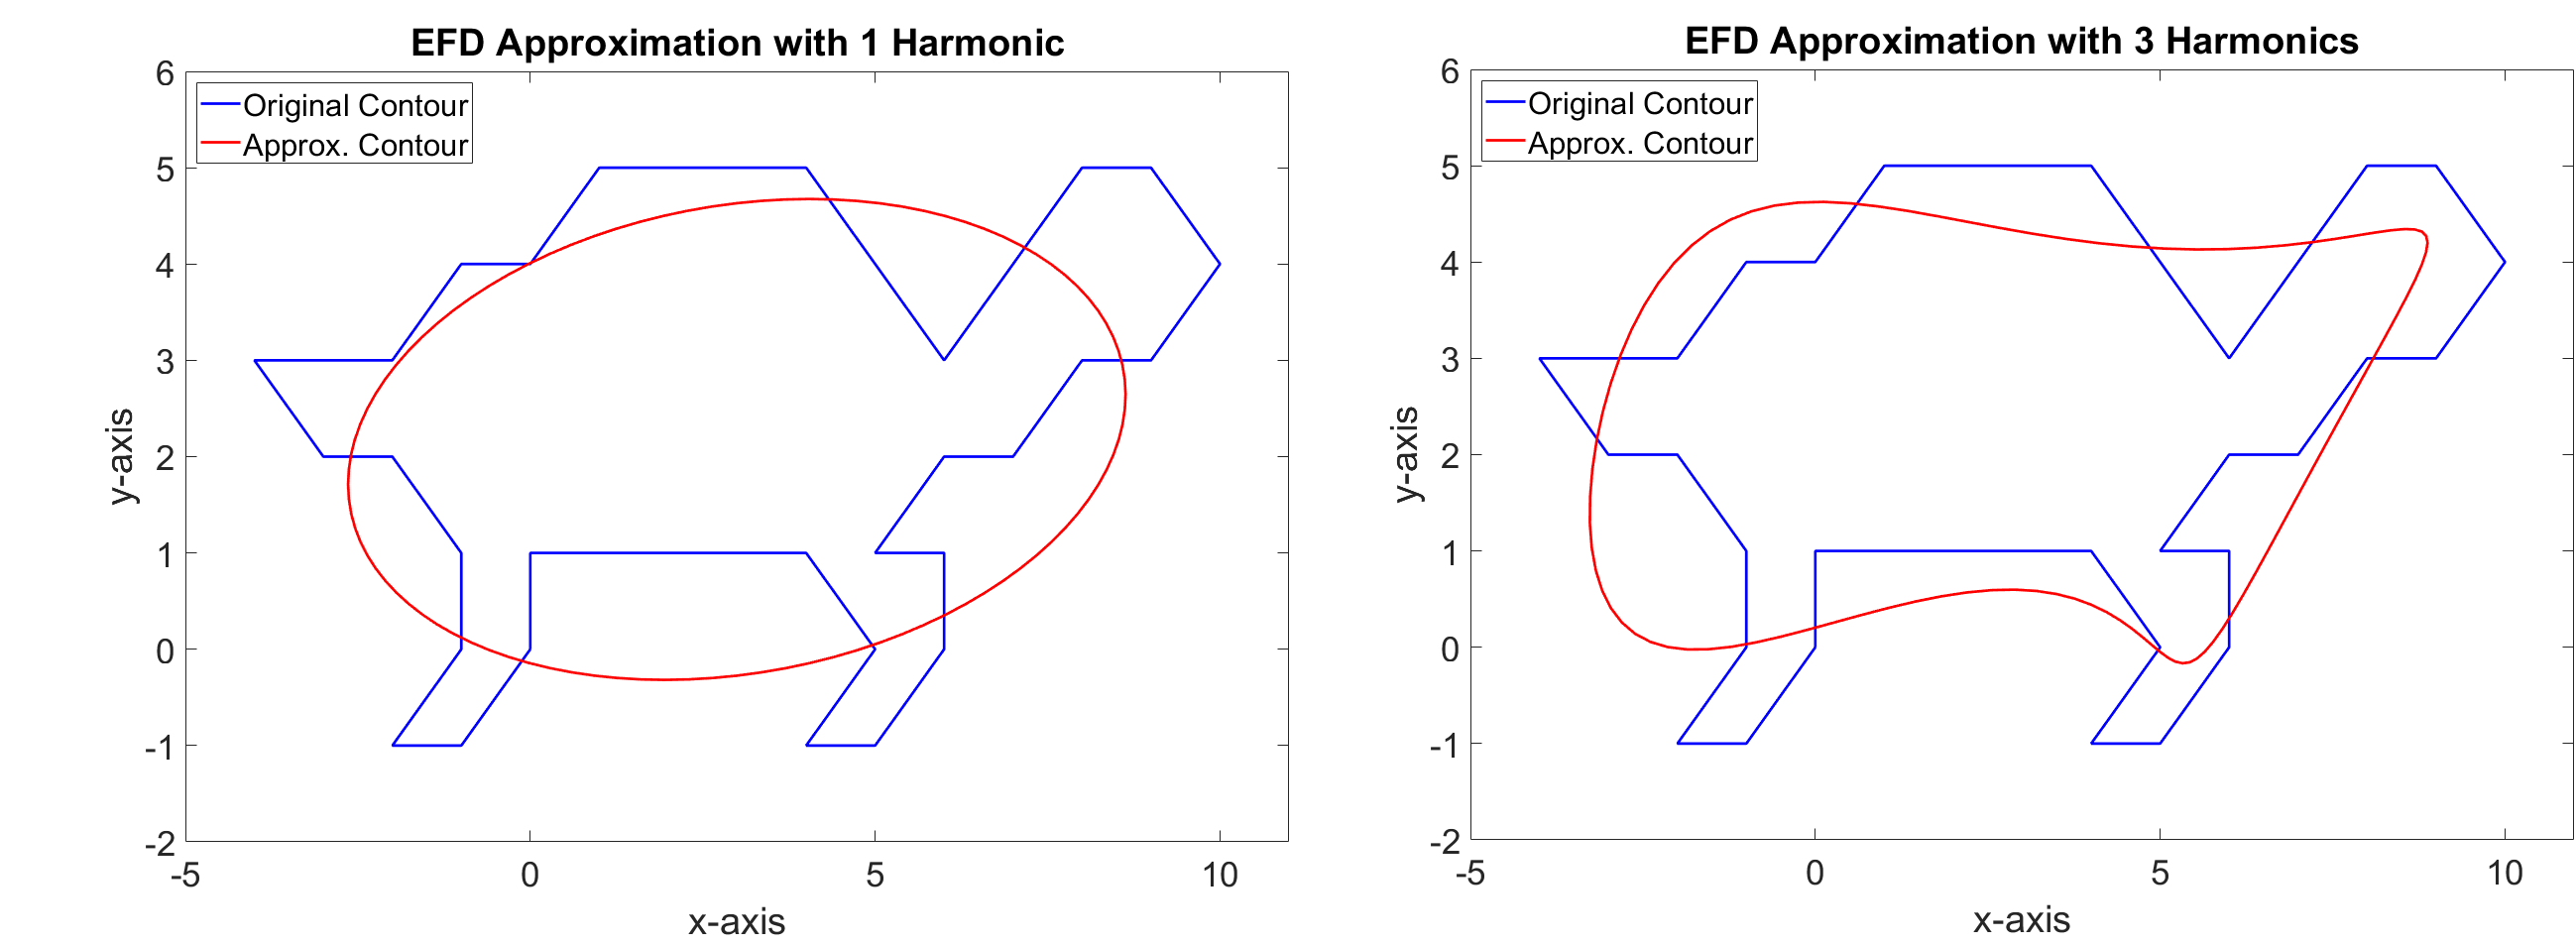
\includegraphics[width=\textwidth,clip, trim=3cm 0cm 0cm 0cm]{efds_1_3.png}		
	\end{subfigure}
	\begin{subfigure}[t]{\textwidth}
		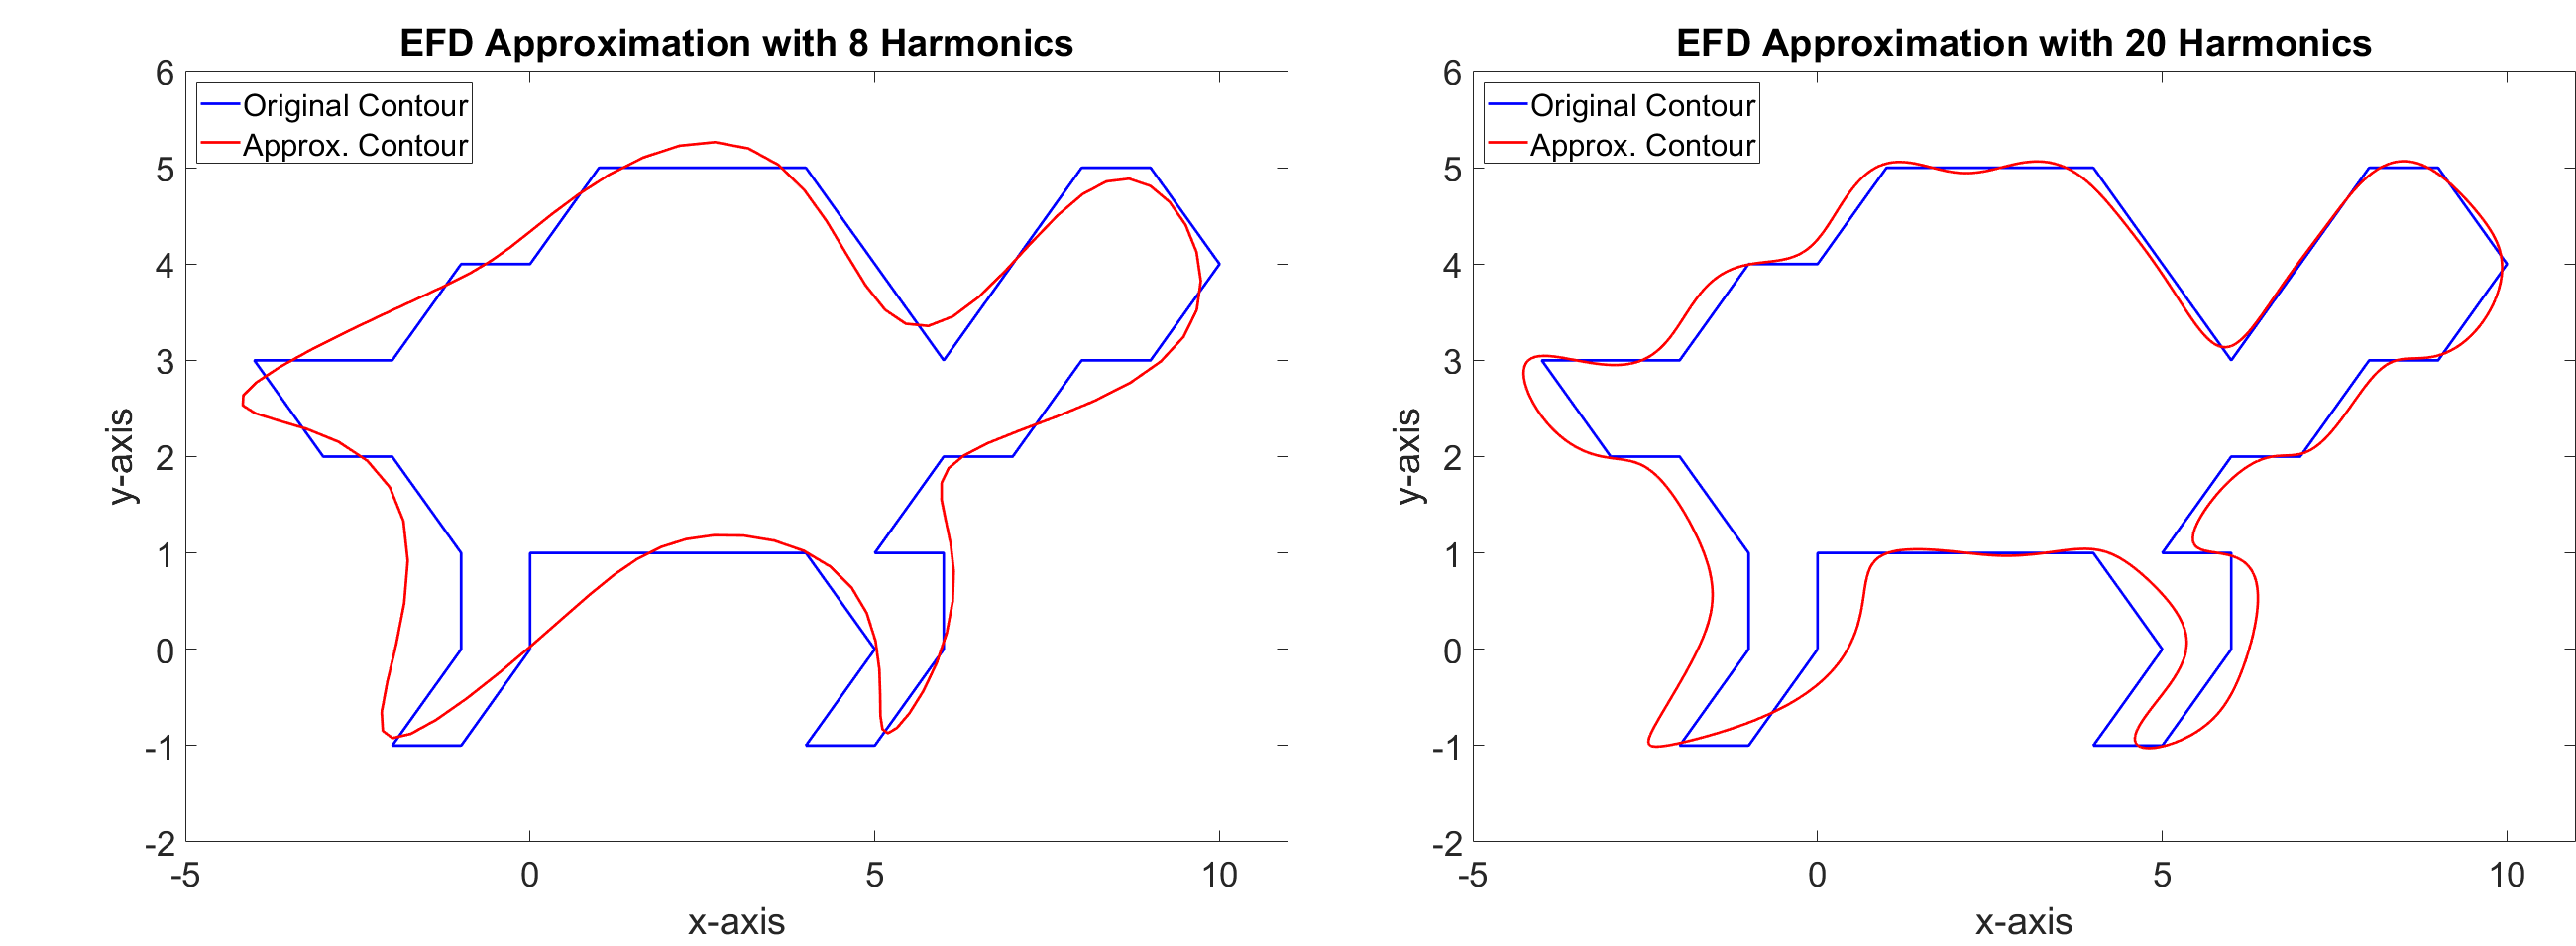
\includegraphics[width=\textwidth,clip, trim=3cm 0cm 0cm 0cm]{efds_8_20.png}		
	\end{subfigure}
	\caption{Approximation of the contour of a cat defined by the freeman chain code 5412343001010007711075454506541344446 using EFDs with 1 Harmonics, 3 Harmonics, 8 Harmonics, and 20 Harmonics. Compared to the original contour, the reconstructed contour is relatively smooth.}
\label{fig:efd_approx}
\end{figure}


\section{Chain Codes} \label{chain_codes}
A contour can be described by the set of it's pixels. However, there are other, often more advantageous, representations for contours. Chain codes are one of those representations. They represent a contour by encoding the relative position of one pixel in the contour to the next contour pixel. By storing the relative positions instead of the absolute pixel positions, translation invariance is achieved \cite{yang2008su}, which is one the advantages of chain codes. Another advantage is that different chain codes can be compared. However, there are two problems of chain codes that make comparison difficult. The first one is that chain codes generally are sensitive to noise \cite{yang2008su}. Another problem is that chain codes usually are not invariant to rotation \cite{yang2008su}. Chain codes are also not invariant to the choosing of the starting pixel \cite{Ballard:1982:CV:578131}, but they can be normalized to be: Choosing a different starting pixel when creating the chain code results in a circular shift of the chain code. To obtain a chain code that is invariant to the choosing of different starting pixels we can circularly shift the chain code until we find the chain code that produces the lowest possible integer \cite{Ballard:1982:CV:578131}. In this thesis we will use chain codes to represent the contour as a one-dimensional signal. This is necessary to apply the fourier transform on the contour. In this section we describe two different chain codes, the freeman chain code and the vertex chain code.    

\subsection{Freeman Chain Code} \label{freeman}
The freeman chain code \cite{freeman} is supposed to be the first chain code that was described. In literature it is often called the basic chain code and used as a representative for all chain codes, because most other chain codes are similar, but use different encoding schemes. \\ A freeman chain code describes a contour by encoding the direction of one contour pixel to the next contour pixel using numbers. The numbers range from 0 to 3 in the case the contour is 4-connected and from 0 to 7 in the case the contour is 8-connected. The specific numbers used for each direction are shown in figure \ref{fig:freeman}. An example of a freeman chain code is shown in figure \ref{FreemanTriangle}. When we use the most left pixel from the figure as a starting pixel, the freeman chain code 111777444444. \\  
There are several advantages to storing freeman chain codes instead of absolute pixel positions. One of those advantages is that freeman chain codes do not require as much memory as absolute pixel positions. For a 4-connected contour we only need to store 2 bits for each chain code element and for an 8-connected contour we only need to store 3 bits for each element of the freeman chain code \cite{Ballard:1982:CV:578131}, because each element can only range from 0 to 3 or from 0 to 7, repectively. Another advantage is that a contour described by a freeman chain code is invariant to translations \cite{yang2008su}. \\
\begin{figure}
	\begin{subfigure}[t]{0.4\textwidth}
		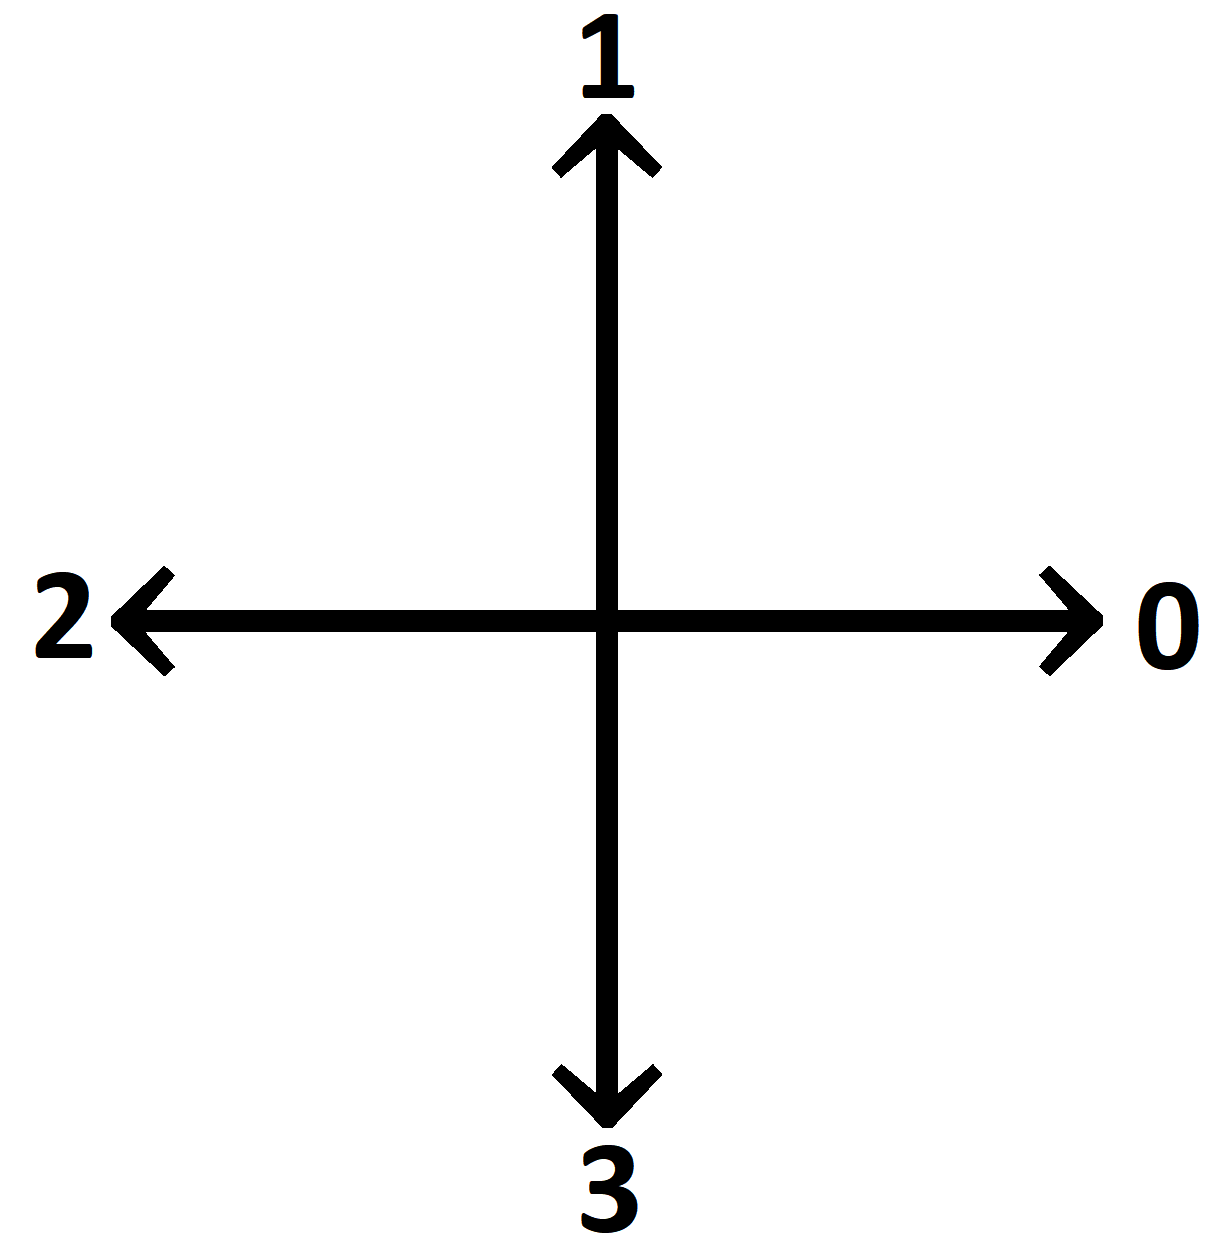
\includegraphics[width=\textwidth]{chaincode4.png}
	\caption{}		
	\end{subfigure}
\hspace{0.1\textwidth}
	\begin{subfigure}[t]{0.4\textwidth}
		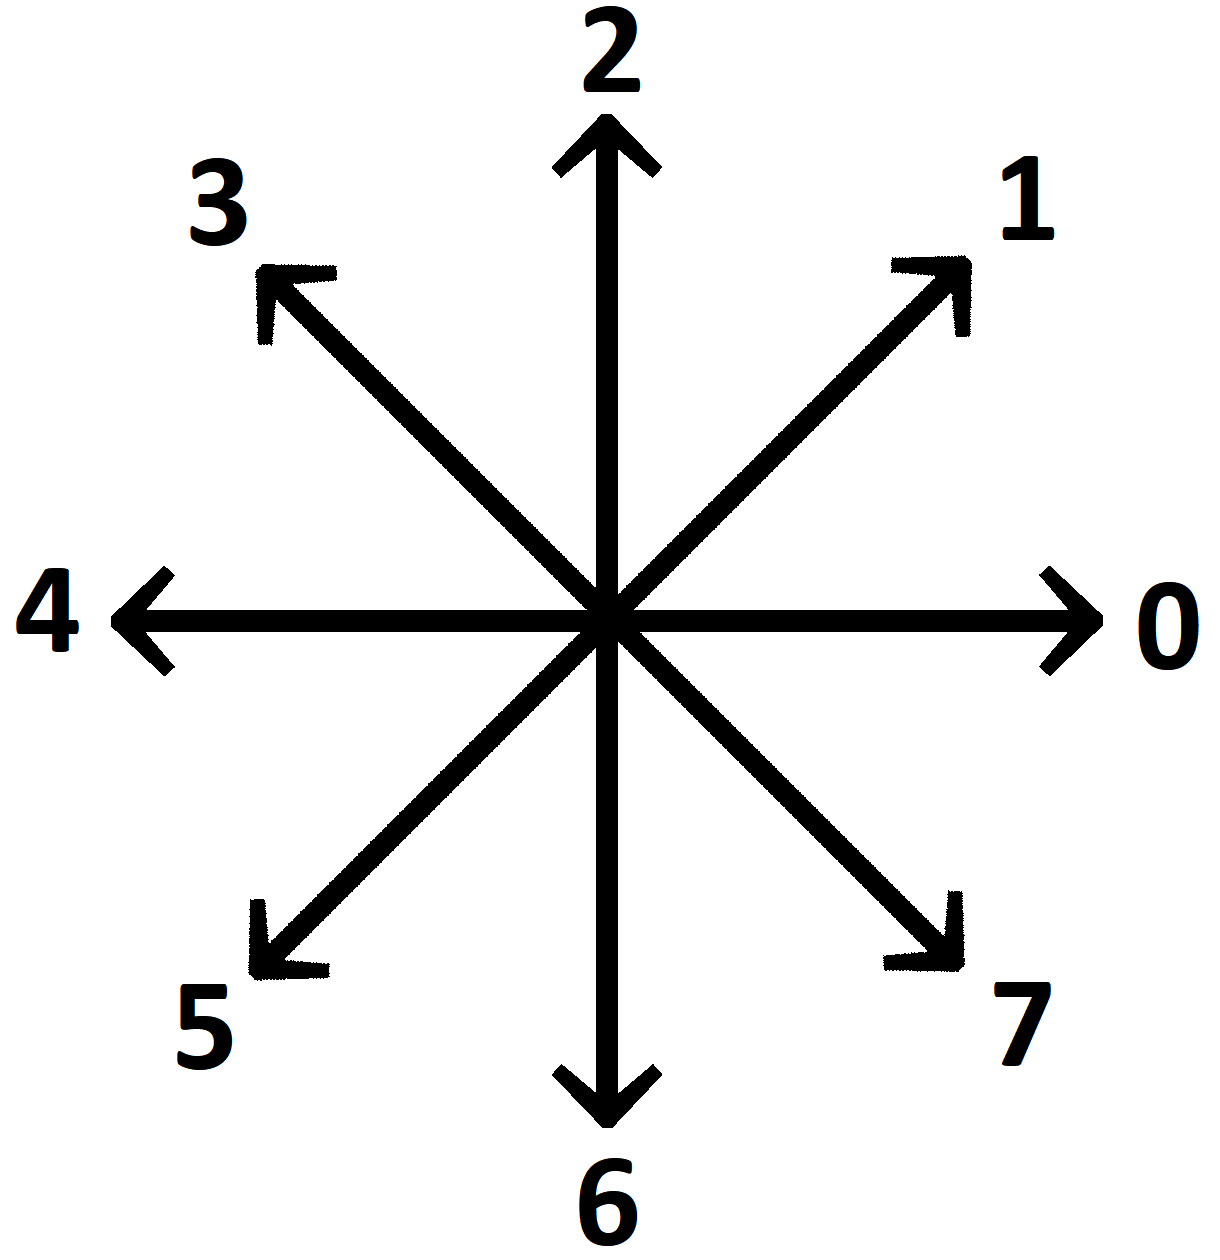
\includegraphics[width=\textwidth]{chaincode.png}		
\caption{}	
	\end{subfigure}
	\caption{Numbers of the freeman chain code  and the corresponding direction they encode for 4-connected (a) and 8-connected (b) contours.}
\label{fig:freeman}
\end{figure}

\textbf{Differential Chain Codes}

 Freeman chain codes are not invariant to rotations \cite{yang2008su,Ballard:1982:CV:578131}. A way to make them invariant to rotations of multiples of 90\si{\degree} is to store the differences of the chain code elements instead of storing the directions from one pixel to the next  \cite{yang2008su}. Computationally, this can be done by subtracting each chain code element from the next and taking the result modulo $n$, where $n$ is the connectivity \cite{yang2008su}. In literature such chain codes are called \textit{differential chain codes} (DCC). As an example of a DCC we use the freeman chain code of the triangle in figure \ref{FreemanTriangle}. The resulting DCC is 006003000003.\\

\newcommand\FreemanExample{
\begin{tikzpicture}
\draw [very thick, draw=black, fill=white] (0,0) grid  (7,4) rectangle (0,0);

%diagonal left to up
\filldraw [fill=gray!50, draw=black, very thick] (0, 0) rectangle (1, 1);
\filldraw [fill=gray!50, draw=black, very thick] (1, 1) rectangle (2, 2);
\filldraw [fill=gray!50, draw=black, very thick] (2, 2) rectangle (3, 3);
\filldraw [fill=gray!50, draw=black, very thick] (3, 3) rectangle (4, 4);

%straight left to right
\filldraw [fill=gray!50, draw=black, very thick] (1, 0) rectangle (2, 1);
\filldraw [fill=gray!50, draw=black, very thick] (2, 0) rectangle (3, 1);
\filldraw [fill=gray!50, draw=black, very thick] (3, 0) rectangle (4, 1);
\filldraw [fill=gray!50, draw=black, very thick] (4, 0) rectangle (5, 1);
\filldraw [fill=gray!50, draw=black, very thick] (5, 0) rectangle (6, 1);
\filldraw [fill=gray!50, draw=black, very thick] (6, 0) rectangle (7, 1);

%diagonal right to up
\filldraw [fill=gray!50, draw=black, very thick] (5, 1) rectangle (6, 2);
\filldraw [fill=gray!50, draw=black, very thick] (4, 2) rectangle (5, 3);

%inner
\filldraw [fill=gray!50, draw=black, very thick] (2, 1) rectangle (3, 2);
\filldraw [fill=gray!50, draw=black, very thick] (3, 1) rectangle (4, 2);
\filldraw [fill=gray!50, draw=black, very thick] (4, 1) rectangle (5, 2);
\filldraw [fill=gray!50, draw=black, very thick] (3, 2) rectangle (4, 3);

%arrows
\draw[draw=black, line width=1.0pt, -Latex] (0.6, 0.6) -- (1.4, 1.4);
\draw[draw=black, line width=1.0pt, -Latex] (1.6, 1.6) -- (2.4, 2.4);
\draw[draw=black, line width=1.0pt, -Latex] (2.6, 2.6) -- (3.4, 3.4);
\draw[draw=black, line width=1.0pt, -Latex] (3.65, 3.35) -- (4.35, 2.65);
\draw[draw=black, line width=1.0pt, -Latex] (4.65, 2.35) -- (5.35, 1.65);
\draw[draw=black, line width=1.0pt, -Latex] (5.65, 1.35) -- (6.35, 0.65);
\draw[draw=black, line width=1.0pt, -Latex] (6.35, 0.5) -- (5.65, 0.5);
\draw[draw=black, line width=1.0pt, -Latex] (5.35, 0.5) -- (4.65, 0.5);
\draw[draw=black, line width=1.0pt, -Latex] (4.35, 0.5) -- (3.65, 0.5);
\draw[draw=black, line width=1.0pt, -Latex] (4.35, 0.5) -- (3.65, 0.5);
\draw[draw=black, line width=1.0pt, -Latex] (3.35, 0.5) -- (2.65, 0.5);
\draw[draw=black, line width=1.0pt, -Latex] (2.35, 0.5) -- (1.65, 0.5);
\draw[draw=black, line width=1.0pt, -Latex] (1.35, 0.5) -- (0.65, 0.5);

%numbers
\node[scale=1.4] at (1.5, 1.5) {1};
\node[scale=1.4] at (2.5, 2.5) {1};
\node[scale=1.4] at (3.5, 3.5) {1};
\node[scale=1.4] at (4.5, 2.5) {7};
\node[scale=1.4] at (5.5, 1.5) {7};
\node[scale=1.4] at (6.5, 0.5) {7};
\node[scale=1.4] at (5.5, 0.5) {4};
\node[scale=1.4] at (4.5, 0.5) {4};
\node[scale=1.4] at (3.5, 0.5) {4};
\node[scale=1.4] at (2.5, 0.5) {4};
\node[scale=1.4] at (1.5, 0.5) {4};
\node[scale=1.4] at (0.5, 0.5) {4};


\end{tikzpicture}
}

\newcommand\VCCExample{
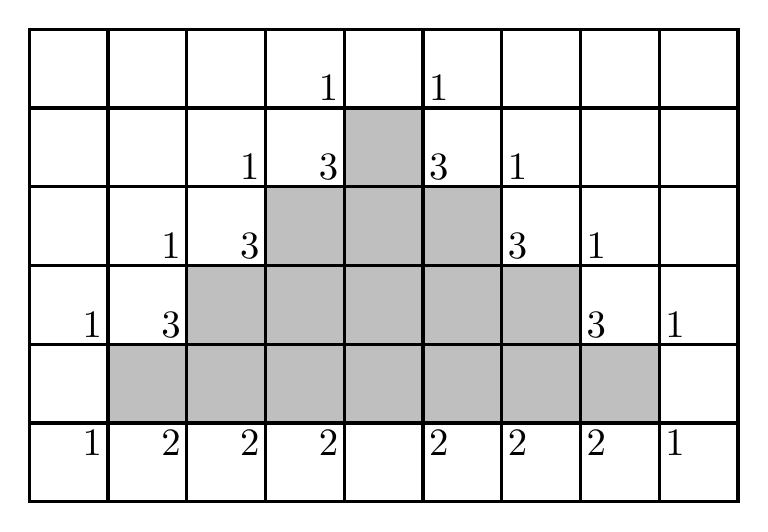
\begin{tikzpicture}
\draw [very thick, draw=black, fill=white] (0,0) grid  (9,6) rectangle (0,0);

%diagonal left to up
\filldraw [fill=gray!50, draw=black, very thick] (1, 1) rectangle (2, 2);
\filldraw [fill=gray!50, draw=black, very thick] (2, 2) rectangle (3, 3);
\filldraw [fill=gray!50, draw=black, very thick] (3, 3) rectangle (4, 4);
\filldraw [fill=gray!50, draw=black, very thick] (4, 4) rectangle (5, 5);

%straight left to right
\filldraw [fill=gray!50, draw=black, very thick] (2, 1) rectangle (3, 2);
\filldraw [fill=gray!50, draw=black, very thick] (3, 1) rectangle (4, 2);
\filldraw [fill=gray!50, draw=black, very thick] (4, 1) rectangle (5, 2);
\filldraw [fill=gray!50, draw=black, very thick] (5, 1) rectangle (6, 2);
\filldraw [fill=gray!50, draw=black, very thick] (6, 1) rectangle (7, 2);
\filldraw [fill=gray!50, draw=black, very thick] (7, 1) rectangle (8, 2);

%diagonal right to up
\filldraw [fill=gray!50, draw=black, very thick] (6, 2) rectangle (7, 3);
\filldraw [fill=gray!50, draw=black, very thick] (5, 3) rectangle (6, 4);

%inner
\filldraw [fill=gray!50, draw=black, very thick] (3, 2) rectangle (4, 3);
\filldraw [fill=gray!50, draw=black, very thick] (4, 2) rectangle (5, 3);
\filldraw [fill=gray!50, draw=black, very thick] (5, 2) rectangle (6, 3);
\filldraw [fill=gray!50, draw=black, very thick] (4, 3) rectangle (5, 4);

\node[scale=1.4] at (0.8, 2.25) {1};
\node[scale=1.4] at (1.8, 2.25) {3};
\node[scale=1.4] at (1.8, 3.25) {1};
\node[scale=1.4] at (2.8, 3.25) {3};
\node[scale=1.4] at (2.8, 4.25) {1};
\node[scale=1.4] at (3.8, 4.25) {3};
\node[scale=1.4] at (3.8, 5.25) {1};
\node[scale=1.4] at (5.2, 5.25) {1};
\node[scale=1.4] at (5.2, 4.25) {3};
\node[scale=1.4] at (6.2, 4.25) {1};
\node[scale=1.4] at (6.2, 3.25) {3};
\node[scale=1.4] at (7.2, 3.25) {1};
\node[scale=1.4] at (7.2, 2.25) {3};
\node[scale=1.4] at (8.2, 2.25) {1};
\node[scale=1.4] at (8.2, 0.75) {1};
\node[scale=1.4] at (7.2, 0.75) {2};
\node[scale=1.4] at (6.2, 0.75) {2};
\node[scale=1.4] at (5.2, 0.75) {2};
\node[scale=1.4] at (3.8, 0.75) {2};
\node[scale=1.4] at (2.8, 0.75) {2};
\node[scale=1.4] at (1.8, 0.75) {2};
\node[scale=1.4] at (0.8, 0.75) {1};
\end{tikzpicture}
}

\begin{figure}
\centering
\begin{minipage}{\textwidth}
\begin{tikzpicture}[font=\small]
\node[draw,inner sep=0pt] (a){\FreemanExample};
\node[draw,inner sep=0pt, right of=a, node distance=9cm] (b){\VCCExample};
\node [below= 1ex of a.south,inner sep=0pt, text width=5cm]{\parbox{\textwidth}{\captionof{subfigure}{Freeman Chain Code\label{FreemanTriangle}}}};
\node [below= 1ex of b.south,inner sep=0pt, text width=5cm]{\parbox{\textwidth}{\captionof{subfigure}{Vertex Chain Code\label{VCCTriangle}}}};
\end{tikzpicture}
\end{minipage}
\caption{Example of the Freeman and Vertex Chain Code.}
 \label{fig:chainCodeExamples}
\end{figure}

\subsection{Vertex Chain Code}
\label{section:vertex_chain_code}
An relatively new chain code is the vertex chain code (VCC) \cite{vertex_chain_code}. The VCC does not follow the pixels as the freeman chain code does. Instead, it follows the vertices that lie on the border between the pixels and the background. The difference becomes more apparent if we consider the chain codes of a single pixel. In such a case the freeman chain code consists of 0 elements. The VCC in this case is 1111. This is because the VCC moves along the 4 edges of the pixel. Each element of the VCC indicates the number of cell vertices, which are in touch with the bounding contour of the shape at that position. Figure \ref{VCCTriangle} shows an example of the VCC. In the figure each vertex on the boundary of the contour corresponds to one chain code element. Another important difference to freeman chain codes is that VCCs are rotation invariant. The VCC can be used for rectangular (pixels), triangle or hexagonal cells. In the following we describe the reconstruction of the boundary of the contour only for the case of rectangular cells, as that is the only case that is relevant in this thesis. In the case of rectangular cells, the element values can be 1, 2, or 3. As can be seen in figure \ref{VCCTriangle} outer corner vertices, vertices on straight contour segments, and inner corner vertices correspond to chain code elements 1, 2, and 3 respectively. \\ To reconstruct a contour described by a VCC several steps have to be done: First each element of the VCC is converted to a \textit{slope change} as defined by the slope change notation in \cite{slope_change_notation}. In the case of rectangular cells this means that the element values 1, 2 and 3 are replaced by 0.5, 0.0, and -0.5 respectively. Then the integral of this slope change chain code is computed, which is the addition of the elements, element by element. For example consider the slope change chain code 1.0 0.5 0.0 -0.5. The first element of the integral is then 1.0. The second element is 1.5 (1.0 + 0.5). The third element is 1.5 (1.0 + 0.5 + 0.0) and the last element is 1.0 (1.0 + 0.5 + 0.0 - 0.5). The finished integral is then 1.0 1.5 1.5 1.0. Each element of the integral can be used to compute the x- and y-displacement from one vertex to the next using the equations in \ref{eq:vcc_reconstruction}. $C_{x_i}$ and $C_{y_i}$ are the displacements described by the $i$-th element in the integral in x- and y-direction respectively. $l$ is the length of one side of a cell. $c_i$ is the current element of the integral. 

\begin{equation} \label{eq:vcc_reconstruction}
\begin{split} 
C_{x_i} = l  cos(\pi c_i) \\
C_{y_i} = l  sin(\pi c_i) \\
\end{split}
\end{equation}



\subfilebib % Makes bibliography available when compiling as subfile
\end{document}